\documentclass[12pt, twoside]{article}
\usepackage[francais]{babel}
\usepackage[T1]{fontenc}
\usepackage[latin1]{inputenc}
\usepackage[left=7mm, right=1cm, top=1cm, bottom=7mm]{geometry}
\usepackage{float}
\usepackage{graphicx}
\usepackage{array} 
\usepackage{multirow}
\usepackage{amsmath,amssymb,mathrsfs}
\usepackage{soul}
\usepackage{textcomp}
\usepackage{eurosym}
\usepackage{variations}
\usepackage{tabvar}

\begin{document}


\ul{Exercice} : 
Construis le sym�trique du segment $[AB]$ par rapport au point $S$ : \\
\begin{center}
	\begin{tabular}{cc} 
		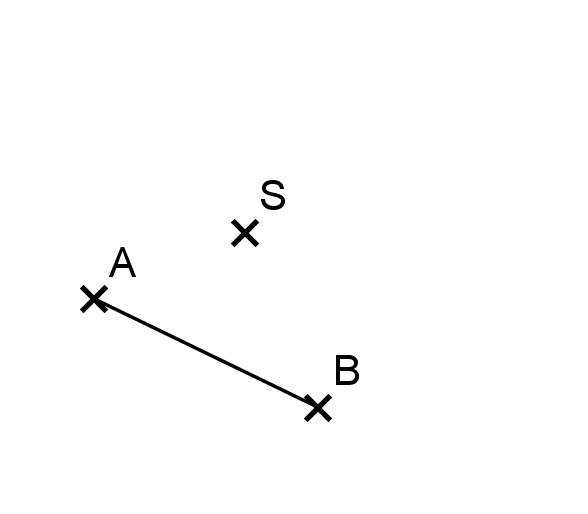
\includegraphics[width=4cm]{images/[AB]01.png} 
		&
		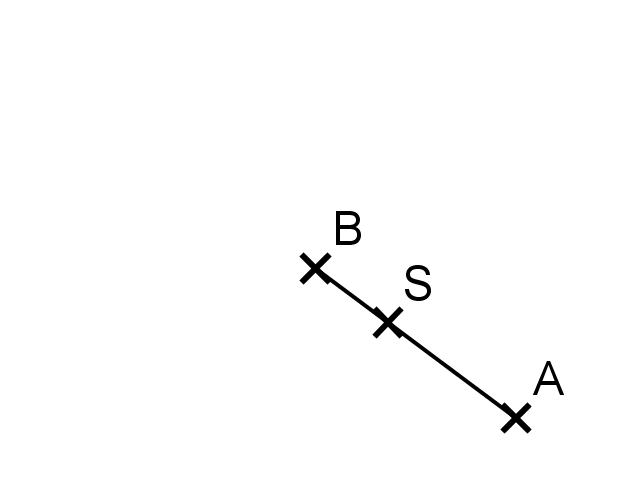
\includegraphics[width=4cm]{images/[AB]02.png} \\
		\qquad & \qquad \\
		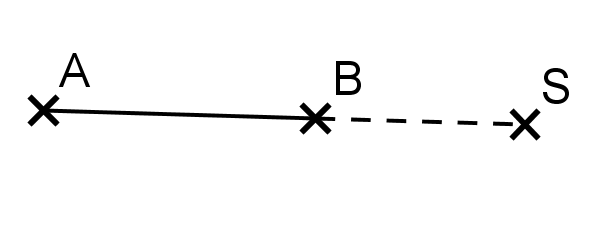
\includegraphics[width=4cm]{images/[AB]03.png} & \\
	\end{tabular}
\end{center}

\bigskip
\ul{Exercice} : 
Construis le symetrie du cercle par rapport au point $T$ : \\
\begin{center}
	\begin{tabular}{ccc} 
		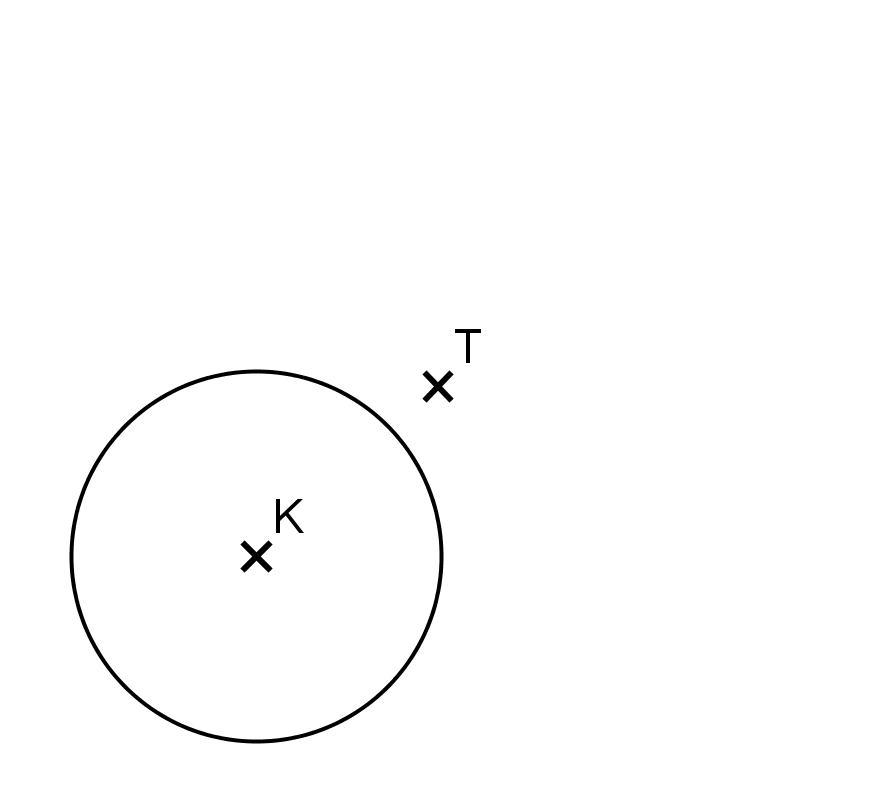
\includegraphics[width=4cm]{images/cercle01.png}
		&
		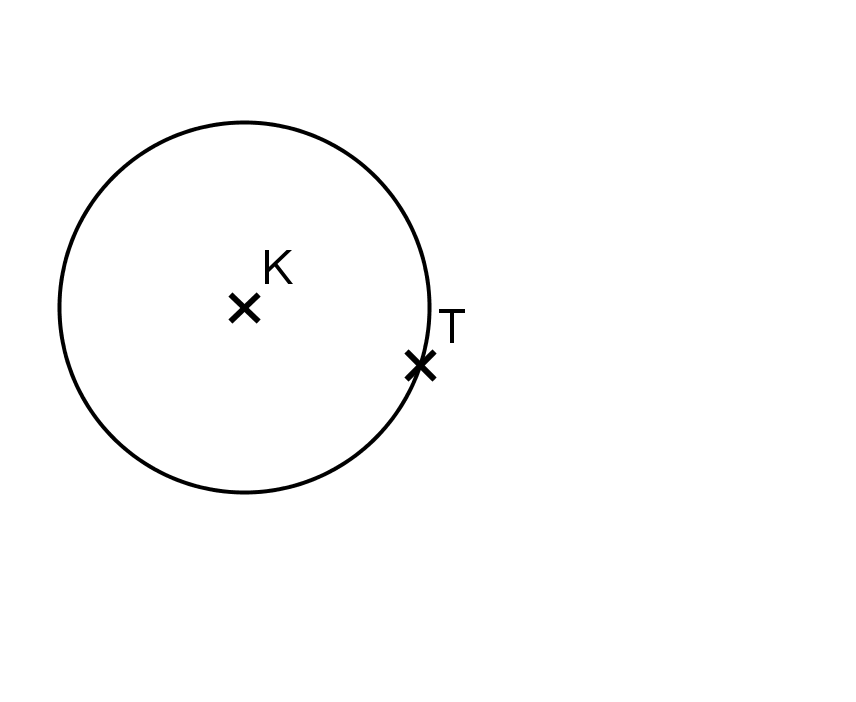
\includegraphics[width=4cm]{images/cercle02.png} 
		&
		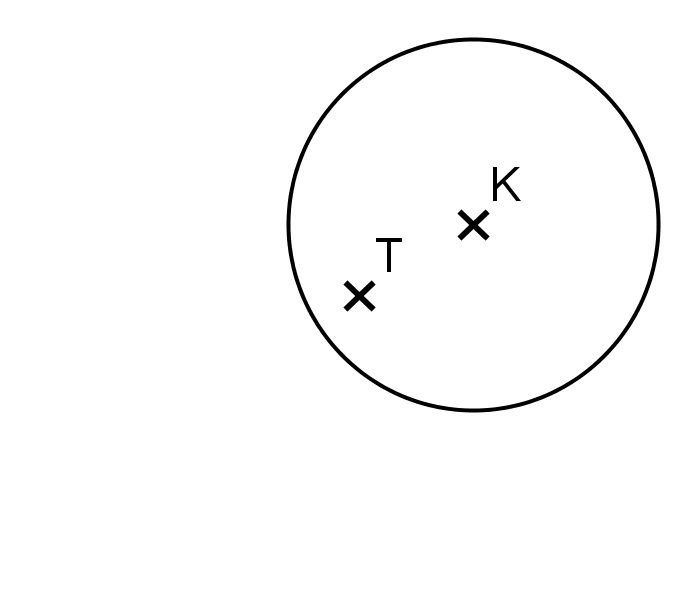
\includegraphics[width=4cm]{images/cercle03.png} 
    \end{tabular}
\end{center}

\bigskip
\ul{Exercice} : 
Construis le sym�trique de la droite $(d)$ par rapport au point $U$ : \\ 
\begin{center}
	\begin{tabular}{ccc} 
		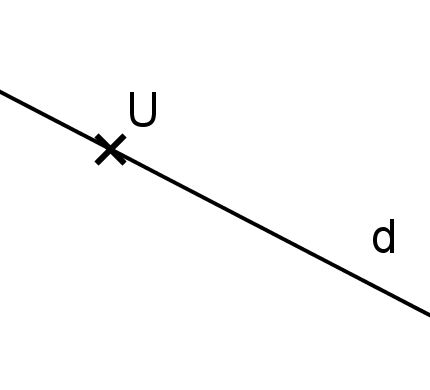
\includegraphics[width=4cm]{images/(d)02.png} 
		& \qquad\qquad\qquad &
		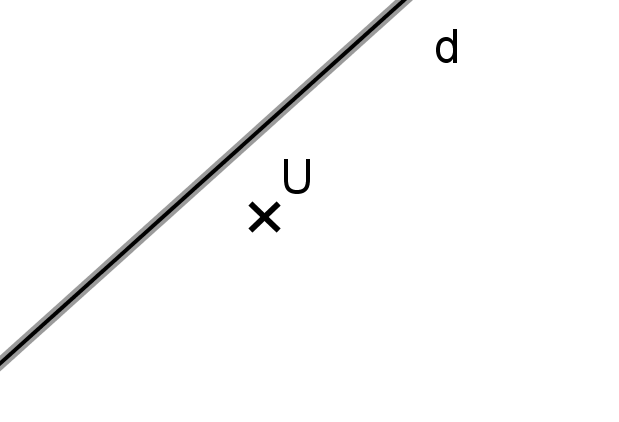
\includegraphics[width=4cm]{images/(d)01.png} 
    \end{tabular}
\end{center}
\end{document}
